\section{Evaluating Depth-Based Tiebreaking}
\label{sec:depth-based-evaluation}

% this text is mostly repeated below, so deleted this and promoted the subsection below up 1 level.
%% We evaluated our depth-based diversifying tiebreaking strategies against standard
%% tiebreaking strategies.
%% In addition to the 35 IPC benchmark domains with 1104 instances used in
%% the previous set of experiments, we used 28 zerocost domains with 620
%% instances.  

%\subsection{Evaluating Depth-Based Tiebreaking with $h$-tiebreaking}

We compared the performance of standard tiebreaking methods to depth-based tiebreaking methods. These all use $h$
as the first-level tiebreaking and either \fifo, \lifo or \ro (random order) as the default tiebreaking criterion
and the only difference is the presence of the third, depth-diversification criteria.

Experiments are conducted on \textbf{1104 standard IPC benchmark
instances} from 35 domains  and \textbf{620 zerocost instances} from 28 domains (see \refsec{sec:eval-common-strategies} and \refsec{sec:zerocost-domains} for full lists of these domains). 
Fundamental experimental setting are the same as the previous ones:
Each experiment uses Fast Downward planner using \astar search and either the \lmcut heuristic or \mands heuristic.
Each experiment is run for 5 minutes excluding SAS translation time, with 4GB memory constraints.

We first show the summary results of these experiments (\reftbl{tbl:depth-summary}).
Overall, depth-based tiebreaking tends to show larger coverages than the
standard tiebreaking strategies.

\begin{table}[htb]
 {
 \centering
 \setlength{\tabcolsep}{3pt}
 \begin{center}
\begin{tabular}{|l|cc|cc|}
Sorting Criteria & Zerocost(620) & Zerocost(620) & IPC(1104) & IPC(1104)\\
 & \lmcut & \mands & \lmcut & \mands\\
Standard &  &  &  & \\
\([f,h,\fifo]\) & 256 & 280 & 558 & 491\\
\([f,h,\lifo]\) & 279 & 301 & 565 & \textbf{496}\\
\([f,h,\ro]\) & 261.9 \(\pm\) 1.4 & 287.7 \(\pm\) 3.2 & 558.9 \(\pm\) 2.1 & 489.4 \(\pm\) 1.0\\
 &  &  &  & \\
Depth-based &  &  &  & \\
\([f,h,\depth,\fifo]\) & 284 & 302 & 571 & 487\\
\([f,h,\depth,\lifo]\) & 264 & 288 & \textbf{575} & 487\\
\([f,h,\depth,\ro]\) & \textbf{288.1 \(\pm\) 1.6} & \textbf{308.1 \(\pm\) 2.1} & 571.4 \(\pm\) 1.7 & 485.6 \(\pm\) 1.5\\
\end{tabular}
\end{center}

 \caption{
 Main summary results: Coverage comparison (number of instances solved in 5min, 4GB, \lmcut/\mands
 heuristics) between standard tiebreaking and depth-based tiebreaking
 ($\depth$). When \lmcut is used, $\depth$ outperforms standard strategies both in IPC
 instances (1104 problems total) and Zerocost instances (620 problems
 total). When \mands is used, $\depth$ outperforms standard strategies
 in Zerocost instances. \textbf{Bold} shows the best configuration.}
 \label{tbl:depth-summary}
 }
\end{table}

Interestingly, when the depth diversity criterion $\depth$ is used, 
the performance relationship between \lifo and \fifo seems to become the opposite:
\fifo tends to perform better than \lifo in zerocost domains for both
\lmcut and \mands heuristics (299 vs 279 for \lmcut, 317 vs 303 for \mands).
Also, \ro (random order) outperforms both \fifo and \lifo.
In the following, we describe and discuss each experiment.

\reftbl{tbl:lmcut-zerocost-full} and \reftbl{tbl:mands-zerocost-full} shows the number of \textbf{620 zerocost
instances} solved by \lmcut and \mands heuristics. In these
zerocost domains, our proposed method outperforms the traditional tiebreaking methods in both heuristics.
Significant improvements were observed in 10 domains when using \lmcut, and in 7 domains when using \mands.
In detail,
\begin{itemize}
 \item \textbf{10 Domains improved by \lmcut on Zerocost} are elevators-up (\ro), freecell-move (\fifo,\ro),
       miconic-up (all), mprime-succumb (\fifo,\ro), pipesnt-pushstart (\ro), pipesworld-pushend (\ro),
       scanalyzer-analyze (\lifo), storage-lift (\fifo), tpp-fuel (\fifo,\ro), woodworking-cut (\fifo,\ro).
 \item \textbf{7 Domains improved by \mands on Zerocost} are elevators-up (\ro), freecell-move (\fifo,\ro),
       mprime-succumb (\fifo,\ro), pipesnt-pushstart (\fifo, \ro), pipesworld-pushend (\ro),
       tpp-fuel (\fifo,\ro), woodworking-cut (\fifo,\ro).
\end{itemize}


\begin{table}[htbp]
 {
 \centering
 \begin{center}
\begin{tabular}{|rHHHHHHHHHHHHcccHHH|cccHHH|}
 & \([f,\fifo]\) & \([f,\lifo]\) & \([f,\ro]\) & R & R & R & \([f,\depth,\fifo]\) & \([f,\depth,\lifo]\) & \([f,\depth,\ro]\) & R & R & R & \([f,h,\fifo]\) & \([f,h,\lifo]\) & \([f,h,\ro]\) & R & R & R & \([f,h,\depth,\fifo]\) & \([f,h,\depth,\lifo]\) & \([f,h,\depth,\ro]\) & R & R & R\\
\hline
 & 227 & 296 & 238.3 \(\pm\) 1.5 & 237 & 238 & 240 & 284 & 276 & 294.7 \(\pm\) 3.1 & 298 & 292 & 294 & 271 & 294 & 276.7 \(\pm\) 1.2 & 276 & 278 & 276 & 299 & 279 & 303.7 \(\pm\) 1.5 & 305 & 304 & 302\\
\hline
airport-fuel(20) & 7 & 15 & 7 \(\pm\) 0 & 7 & 7 & 7 & 10 & 13 & 10.3 \(\pm\) 0.6 & 10 & 10 & 11 & 15 & 13 & 13.7 \(\pm\) 0.6 & 13 & 14 & 14 & 14 & 13 & 14 \(\pm\) 0 & 14 & 14 & 14\\
blocks-stack(20) & 15 & 17 & 15 \(\pm\) 0 & 15 & 15 & 15 & 17 & 18 & 17.7 \(\pm\) 0.6 & 18 & 18 & 17 & 17 & 17 & 17 \(\pm\) 0 & 17 & 17 & 17 & 17 & 17 & 17 \(\pm\) 0 & 17 & 17 & 17\\
depot-fuel(22) & 4 & 6 & 5.3 \(\pm\) 0.6 & 5 & 5 & 6 & 6 & 6 & 6 \(\pm\) 0 & 6 & 6 & 6 & 6 & 6 & 6 \(\pm\) 0 & 6 & 6 & 6 & 6 & 6 & 6 \(\pm\) 0 & 6 & 6 & 6\\
driverlog-fuel(20) & 7 & 8 & 7 \(\pm\) 0 & 7 & 7 & 7 & 8 & 8 & 8 \(\pm\) 0 & 8 & 8 & 8 & 8 & 8 & 8 \(\pm\) 0 & 8 & 8 & 8 & 8 & 8 & 8 \(\pm\) 0 & 8 & 8 & 8\\
elevators-up(20) & 7 & 13 & 7 \(\pm\) 0 & 7 & 7 & 7 & 7 & 9 & 8.7 \(\pm\) 0.6 & 9 & 9 & 8 & 7 & 13 & 7 \(\pm\) 0 & 7 & 7 & 7 & 7 & 9 & 8.7 \(\pm\) 0.6 & 9 & 9 & 8\\
floortile-ink(20) & 8 & 8 & 8 \(\pm\) 0 & 8 & 8 & 8 & 8 & 8 & 8 \(\pm\) 0 & 8 & 8 & 8 & 8 & 8 & 8.3 \(\pm\) 0.6 & 9 & 8 & 8 & 8 & 8 & 8.3 \(\pm\) 0.6 & 9 & 8 & 8\\
freecell-move(20) & 4 & 19 & 5 \(\pm\) 0 & 5 & 5 & 5 & 17 & 10 & 16.7 \(\pm\) 0.6 & 17 & 16 & 17 & 4 & 19 & 5 \(\pm\) 0 & 5 & 5 & 5 & 17 & 10 & 16.3 \(\pm\) 0.6 & 17 & 16 & 16\\
 & 15 & 15 & 15 \(\pm\) 0 & 15 & 15 & 15 & 13 & 15 & 14.7 \(\pm\) 0.6 & 15 & 15 & 14 & 15 & 15 & 15 \(\pm\) 0 & 15 & 15 & 15 & 15 & 15 & 15 \(\pm\) 0 & 15 & 15 & 15\\
grid-fuel(5) & 1 & 1 & 1 \(\pm\) 0 & 1 & 1 & 1 & 1 & 1 & 1 \(\pm\) 0 & 1 & 1 & 1 & 1 & 1 & 1 \(\pm\) 0 & 1 & 1 & 1 & 1 & 1 & 1 \(\pm\) 0 & 1 & 1 & 1\\
gripper-move(20) & 7 & 7 & 7 \(\pm\) 0 & 7 & 7 & 7 & 7 & 7 & 7 \(\pm\) 0 & 7 & 7 & 7 & 7 & 7 & 7 \(\pm\) 0 & 7 & 7 & 7 & 7 & 7 & 7 \(\pm\) 0 & 7 & 7 & 7\\
hiking-fuel(20) & 8 & 9 & 8 \(\pm\) 0 & 8 & 8 & 8 & 9 & 9 & 9 \(\pm\) 0 & 9 & 9 & 9 & 9 & 9 & 9 \(\pm\) 0 & 9 & 9 & 9 & 9 & 9 & 9 \(\pm\) 0 & 9 & 9 & 9\\
logistics00-fuel(28) & 15 & 16 & 15 \(\pm\) 0 & 15 & 15 & 15 & 15 & 16 & 15 \(\pm\) 0 & 15 & 15 & 15 & 16 & 16 & 16 \(\pm\) 0 & 16 & 16 & 16 & 16 & 16 & 15.3 \(\pm\) 0.6 & 16 & 15 & 15\\
miconic-up(30) & 10 & 17 & 10 \(\pm\) 0 & 10 & 10 & 10 & 19 & 18 & 19.3 \(\pm\) 1.2 & 20 & 20 & 18 & 16 & 17 & 16.7 \(\pm\) 0.6 & 16 & 17 & 17 & 19 & 18 & 20.3 \(\pm\) 0.6 & 20 & 21 & 20\\
mprime-succumb(35) & 12 & 14 & 11.3 \(\pm\) 1.2 & 10 & 12 & 12 & 21 & 14 & 19.7 \(\pm\) 1.2 & 19 & 19 & 21 & 15 & 14 & 16.7 \(\pm\) 0.6 & 17 & 17 & 16 & 22 & 14 & 20.3 \(\pm\) 0.6 & 20 & 20 & 21\\
mystery-feast(20) & 5 & 5 & 6.3 \(\pm\) 1.2 & 7 & 5 & 7 & 6 & 7 & 6.3 \(\pm\) 0.6 & 7 & 6 & 6 & 7 & 5 & 7.7 \(\pm\) 0.6 & 7 & 8 & 8 & 6 & 5 & 7.3 \(\pm\) 1.5 & 6 & 9 & 7\\
nomystery-fuel(20) & 9 & 10 & 9 \(\pm\) 0 & 9 & 9 & 9 & 9 & 10 & 9.3 \(\pm\) 0.6 & 10 & 9 & 9 & 10 & 10 & 10 \(\pm\) 0 & 10 & 10 & 10 & 10 & 10 & 10 \(\pm\) 0 & 10 & 10 & 10\\
parking-movecc(20) & 0 & 0 & 0 \(\pm\) 0 & 0 & 0 & 0 & 0 & 0 & 0 \(\pm\) 0 & 0 & 0 & 0 & 0 & 0 & 0 \(\pm\) 0 & 0 & 0 & 0 & 0 & 0 & 0 \(\pm\) 0 & 0 & 0 & 0\\
pathways-fuel(30) & 4 & 5 & 4 \(\pm\) 0 & 4 & 4 & 4 & 4 & 5 & 4.3 \(\pm\) 0.6 & 4 & 5 & 4 & 5 & 5 & 4.7 \(\pm\) 0.6 & 5 & 5 & 4 & 5 & 5 & 4.3 \(\pm\) 0.6 & 5 & 4 & 4\\
pipesnt-pushstart(20) & 6 & 7 & 8.3 \(\pm\) 0.6 & 8 & 8 & 9 & 8 & 6 & 10 \(\pm\) 0 & 10 & 10 & 10 & 8 & 8 & 8.3 \(\pm\) 0.6 & 8 & 8 & 9 & 8 & 8 & 10 \(\pm\) 0 & 10 & 10 & 10\\
pipesworld-pushend(20) & 2 & 4 & 2.7 \(\pm\) 0.6 & 3 & 3 & 2 & 4 & 3 & 5.3 \(\pm\) 0.6 & 6 & 5 & 5 & 3 & 4 & 3.7 \(\pm\) 0.6 & 4 & 4 & 3 & 3 & 3 & 5 \(\pm\) 0 & 5 & 5 & 5\\
psr-small-open(20) & 19 & 19 & 19 \(\pm\) 0 & 19 & 19 & 19 & 19 & 19 & 19 \(\pm\) 0 & 19 & 19 & 19 & 19 & 19 & 19 \(\pm\) 0 & 19 & 19 & 19 & 19 & 19 & 19 \(\pm\) 0 & 19 & 19 & 19\\
rovers-fuel(40) & 7 & 9 & 7 \(\pm\) 0 & 7 & 7 & 7 & 8 & 9 & 9 \(\pm\) 0 & 9 & 9 & 9 & 8 & 8 & 8 \(\pm\) 0 & 8 & 8 & 8 & 8 & 8 & 8 \(\pm\) 0 & 8 & 8 & 8\\
scanalyzer-analyze(20) & 3 & 9 & 3 \(\pm\) 0 & 3 & 3 & 3 & 6 & 5 & 5 \(\pm\) 0 & 5 & 5 & 5 & 9 & 9 & 9 \(\pm\) 0 & 9 & 9 & 9 & 9 & 10 & 9.3 \(\pm\) 0.6 & 10 & 9 & 9\\
sokoban-pushgoal(20) & 18 & 18 & 18 \(\pm\) 0 & 18 & 18 & 18 & 18 & 18 & 17.7 \(\pm\) 0.6 & 18 & 17 & 18 & 18 & 18 & 18 \(\pm\) 0 & 18 & 18 & 18 & 18 & 18 & 18 \(\pm\) 0 & 18 & 18 & 18\\
storage-lift(20) & 4 & 4 & 4 \(\pm\) 0 & 4 & 4 & 4 & 5 & 5 & 5 \(\pm\) 0 & 5 & 5 & 5 & 4 & 4 & 4 \(\pm\) 0 & 4 & 4 & 4 & 5 & 4 & 4 \(\pm\) 0 & 4 & 4 & 4\\
tidybot-motion(20) & 14 & 16 & 14.7 \(\pm\) 0.6 & 14 & 15 & 15 & 15 & 15 & 16 \(\pm\) 0 & 16 & 16 & 16 & 16 & 16 & 16 \(\pm\) 0 & 16 & 16 & 16 & 16 & 16 & 16 \(\pm\) 0 & 16 & 16 & 16\\
tpp-fuel(30) & 7 & 11 & 8 \(\pm\) 0 & 8 & 8 & 8 & 10 & 10 & 11 \(\pm\) 0 & 11 & 11 & 11 & 8 & 11 & 8 \(\pm\) 0 & 8 & 8 & 8 & 11 & 10 & 11 \(\pm\) 0 & 11 & 11 & 11\\
woodworking-cut(20) & 2 & 7 & 5.7 \(\pm\) 0.6 & 6 & 6 & 5 & 7 & 5 & 8.7 \(\pm\) 1.5 & 9 & 7 & 10 & 5 & 7 & 7 \(\pm\) 0 & 7 & 7 & 7 & 8 & 5 & 8.3 \(\pm\) 0.6 & 8 & 8 & 9\\
zenotravel-fuel(20) & 7 & 7 & 7 \(\pm\) 0 & 7 & 7 & 7 & 7 & 7 & 7 \(\pm\) 0 & 7 & 7 & 7 & 7 & 7 & 7 \(\pm\) 0 & 7 & 7 & 7 & 7 & 7 & 7 \(\pm\) 0 & 7 & 7 & 7\\
\end{tabular}
\end{center}

 % 
  \caption{ Coverage comparison (the number of instances solved in 5min, 4GB, \lmcut heuristics) on \textbf{620
 zerocost instances}.  We highlight the best results when the difference between the best and the worst coverages
 is greater than 2.  }
 % 
 \label{tbl:lmcut-zerocost-full}}
\end{table}

\begin{table}[htbp]
 {
 \centering
 \begin{center}
\begin{tabular}{|c|cccHHH|cccHHH|cccHHH|cccHHH|}
zerocost & mn\_$_{\text{F27958}}$ & mn\_$_{\text{L28267}}$ & mn\_$_{\text{R10848}}$ & mn\_$_{\text{R2894}}$ & mn\_$_{\text{R7102}}$ & mn$_{\text{iF27958}}$ & mn$_{\text{iL28267}}$ & mn$_{\text{iR10848}}$ & mn$_{\text{iR2894}}$ & mn$_{\text{iR7102}}$ & mnh$_{\text{F27958}}$ & mnh$_{\text{L28267}}$ & mnh$_{\text{R10848}}$ & mnh$_{\text{R2894}}$ & mnh$_{\text{R7102}}$ & mnhiF27958 & mnhiL28267 & mnhiR10848 & mnhiR2894 & mnhiR7102\\
cov & 250 & 315 & 269 & 271 & 270 & 310 & 289 & 317 & 314 & 317 & 295 & 316 & 304 & 304 & 304 & 317 & 303 & 326 & 322 & 326\\
rprt & 5 & 5 & 5 & 5 & 5 & 5 & 5 & 5 & 5 & 5 & 5 & 5 & 5 & 5 & 5 & 5 & 5 & 5 & 5 & 5\\
blck & 20 & 20 & 20 & 20 & 20 & 20 & 20 & 20 & 20 & 20 & 20 & 20 & 20 & 20 & 20 & 20 & 20 & 20 & 20 & 20\\
dpt- & 5 & 5 & 6 & 6 & 6 & 6 & 5 & 6 & 6 & 6 & 5 & 5 & 6 & 6 & 6 & 6 & 5 & 6 & 6 & 6\\
drvr & 8 & 9 & 8 & 8 & 8 & 9 & 9 & 9 & 9 & 9 & 9 & 9 & 9 & 9 & 9 & 9 & 9 & 9 & 9 & 9\\
lvtr & 8 & 14 & 8 & 8 & 9 & 9 & 13 & 12 & 12 & 10 & 8 & 14 & 8 & 8 & 9 & 9 & 13 & 12 & 12 & 10\\
flrt & 8 & 8 & 8 & 8 & 8 & 7 & 8 & 7 & 7 & 8 & 8 & 8 & 8 & 8 & 8 & 7 & 7 & 7 & 7 & 6\\
frcl & 5 & 17 & 8 & 7 & 6 & 17 & 15 & 17 & 17 & 17 & 5 & 17 & 8 & 7 & 6 & 17 & 15 & 17 & 17 & 17\\
gd-p & 15 & 15 & 15 & 15 & 15 & 15 & 15 & 15 & 15 & 15 & 15 & 15 & 15 & 15 & 15 & 15 & 15 & 15 & 15 & 15\\
grd- & 2 & 2 & 2 & 2 & 2 & 2 & 2 & 2 & 2 & 2 & 2 & 2 & 2 & 2 & 2 & 2 & 2 & 2 & 2 & 2\\
grpp & 8 & 20 & 8 & 8 & 8 & 20 & 10 & 18 & 18 & 19 & 20 & 20 & 20 & 20 & 20 & 20 & 20 & 20 & 20 & 20\\
hkng & 12 & 13 & 12 & 12 & 13 & 13 & 12 & 12 & 12 & 12 & 13 & 13 & 13 & 13 & 13 & 13 & 12 & 12 & 13 & 12\\
lgst & 16 & 16 & 16 & 16 & 16 & 16 & 16 & 16 & 16 & 16 & 16 & 16 & 16 & 16 & 16 & 16 & 16 & 16 & 16 & 16\\
mcnc & 19 & 30 & 19 & 20 & 20 & 30 & 30 & 30 & 30 & 30 & 29 & 30 & 30 & 30 & 30 & 30 & 30 & 30 & 30 & 30\\
mprm & 14 & 19 & 15 & 16 & 15 & 24 & 15 & 22 & 20 & 22 & 21 & 19 & 20 & 19 & 20 & 25 & 15 & 24 & 22 & 25\\
myst & 4 & 4 & 6 & 6 & 6 & 4 & 4 & 6 & 6 & 6 & 4 & 4 & 6 & 6 & 6 & 4 & 4 & 6 & 6 & 6\\
nmys & 15 & 16 & 16 & 16 & 16 & 15 & 16 & 16 & 16 & 16 & 16 & 16 & 16 & 16 & 16 & 16 & 16 & 16 & 16 & 16\\
prkn & 0 & 0 & 0 & 0 & 0 & 0 & 0 & 0 & 0 & 0 & 0 & 0 & 0 & 0 & 0 & 0 & 0 & 0 & 0 & 0\\
pthw & 4 & 4 & 4 & 4 & 4 & 4 & 4 & 4 & 4 & 4 & 4 & 4 & 4 & 4 & 4 & 4 & 4 & 4 & 4 & 4\\
ppsn & 3 & 3 & 3 & 4 & 3 & 5 & 3 & 5 & 5 & 5 & 3 & 3 & 3 & 4 & 3 & 5 & 3 & 5 & 5 & 5\\
ppsw & 3 & 9 & 7 & 8 & 8 & 4 & 4 & 9 & 8 & 9 & 5 & 9 & 8 & 8 & 8 & 5 & 6 & 9 & 8 & 10\\
psr- & 19 & 19 & 19 & 19 & 19 & 19 & 19 & 19 & 19 & 19 & 19 & 19 & 19 & 19 & 19 & 19 & 19 & 19 & 19 & 19\\
rvrs & 8 & 8 & 8 & 8 & 8 & 8 & 8 & 8 & 8 & 8 & 8 & 8 & 8 & 8 & 8 & 8 & 8 & 8 & 8 & 8\\
scnl & 9 & 11 & 9 & 9 & 9 & 9 & 9 & 9 & 9 & 8 & 11 & 11 & 11 & 11 & 11 & 11 & 11 & 11 & 11 & 11\\
skbn & 18 & 18 & 19 & 18 & 18 & 18 & 18 & 17 & 17 & 17 & 19 & 19 & 18 & 18 & 19 & 18 & 18 & 18 & 18 & 18\\
strg & 4 & 4 & 4 & 4 & 4 & 4 & 4 & 4 & 4 & 4 & 4 & 4 & 4 & 4 & 4 & 4 & 4 & 4 & 4 & 4\\
tdyb & 0 & 0 & 0 & 0 & 0 & 0 & 0 & 0 & 0 & 0 & 0 & 0 & 0 & 0 & 0 & 0 & 0 & 0 & 0 & 0\\
tpp- & 8 & 10 & 8 & 8 & 8 & 11 & 10 & 11 & 11 & 11 & 9 & 10 & 9 & 10 & 9 & 11 & 10 & 11 & 11 & 11\\
wdwr & 2 & 7 & 7 & 7 & 7 & 7 & 6 & 9 & 9 & 9 & 7 & 7 & 8 & 8 & 8 & 8 & 7 & 10 & 8 & 11\\
zntr & 8 & 9 & 9 & 9 & 9 & 9 & 9 & 9 & 9 & 10 & 10 & 9 & 10 & 10 & 10 & 10 & 9 & 10 & 10 & 10\\
\end{tabular}
\end{center}

  \caption{
 Coverage comparison (the number of instances solved in 5min, 4GB, \mands heuristics)
 on \textbf{620 zerocost instances}. We highlight the
 best results when the difference between the maximum and the minimum coverage exceeds 2.
 }
 \label{tbl:mands-zerocost-full}
 }
\end{table}

\reftbl{tbl:lmcut-ipc-full} shows the number of \textbf{1104 standard IPC benchmark instances} solved by \lmcut
heuristics. Depth-based tiebreaking ($\depth$) shows impressive results on \pddl{Openstacks} ($\fifo:2\to 8,\ \lifo:3\to 12,\  \ro:3.9\to 10$) and \pddl{Cybersec} ($\fifo: 11\to 18,\ \ro: 11.7\to 18$) because these
domains contain many instances of zero-cost edges and the final plateau $\plateau{f,h}$ is huge (See
\refig{fig:plateau}).  Most other instances are unaffected by depth-based tiebreaking.  Thus, depth-based
tie-breaking yields better performance in the domains with large final plateaus, without sacrificing performance in
other domains.

In contrast, \reftbl{tbl:mands-ipc-full} shows that depth-based tiebreaking negatively affects the performance of
\mands when applied to \textbf{1104 standard IPC benchmark instances}. Our justification to this result is
the following.
% 
First, the coverage of \pddl{Openstacks} is improved in \fifo ($15\to 19$) and \ro ($15.4\to 19$), so we have achieved the expected behavior.
%
While it did not happened to \pddl{Cybersec}, this is due to the poor performance of \mands in \pddl{Cybersec}.
The coverage of \pddl{Cybersec} is 0 in all configurations and even depth could not improve it. Thus, the positive
effect of depth diversification to the overall score was limited.
% 
Second, we observed a performance degradation across wide range of domains which is caused by the low-level overhead of depth-based tiebreaking (i.e., updates to the depth-based bucket data structures).
As shown in \refig{fig:expansion-ratio}, the number of evaluation of \mands heuristics per seconds has significantly decreased across wide range of domains, while such effect is limited in \lmcut.
This is because the evaluation of \mands heuristics is implemented
as an efficient table lookup, and it is able to evaluate an order of magnitude larger number of nodes compared to \lmcut heuristics.
Thus, even the relatively small overhead incurred by the management of depth buckets decreases the node evaluation rate sufficiently to noticeably degrade performance.
In contrast, \mands did not have such problems in Zerocost domains. This shows that the search efficiency offered by depth based diversification become much more important, and the overhead caused by the management of depth buckets become negligible even in the case of \mands.

% , which is less interesting when tackling an intractable combinatorial problems.

\begin{figure}[htbp]
 \centering
 % \begin{tabular}{cccc}
 %  nodes/sec                  & LMcut      & M\&S       & M\&S slowdown\\
 %  \hline
 %  $[f,h,\lifo]$              & 8.86$\times 10^3$ & 1.37$\times 10^5$ & 100\%\\
 %  $[f,h,\depth,\lifo]$ & 9.37$\times 10^3$ & 1.13$\times 10^5$ & 82\%\\
 %  \hline
 %  $[f,h,\fifo]$              & 9.65$\times 10^3$ & 1.41$\times 10^5$ & 100\%\\
 %  $[f,h,\depth,\fifo]$ & 9.62$\times 10^3$ & 1.24$\times 10^5$ & 87\%\\
 %  \hline
 % \end{tabular}
 % \caption{Comparison of the average node expansion ratio (node/sec) between
 % standard tiebreaking and depth-based tiebreaking on \lmcut and \mands
 % heuristics. Numbers are averaged over the problem instances solved by
 % all 4 configurations. Since the node evaluation of \mands is an order of
 % magnitude faster than \lmcut, the overhead of managing depth-based
 % tiebreaking queue is non-negligible on \mands.}
 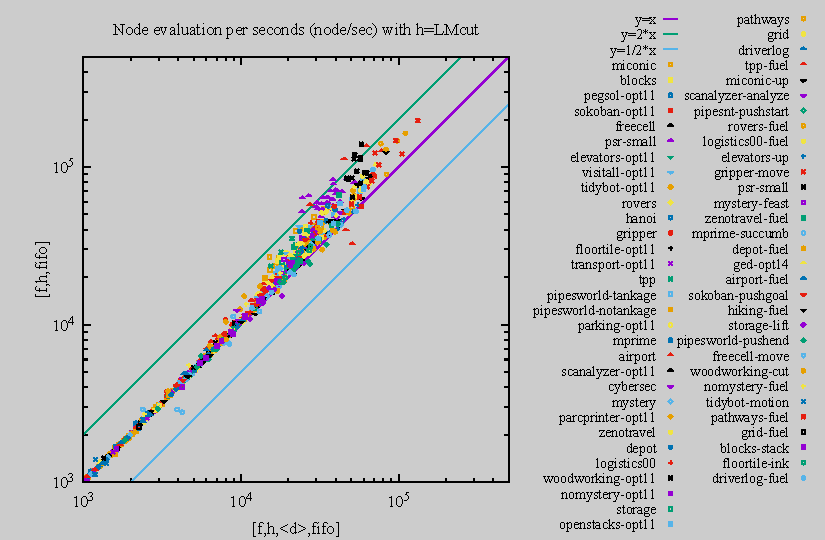
\includegraphics{img/node-sec/lmhiF-lmh_F.pdf}
 % 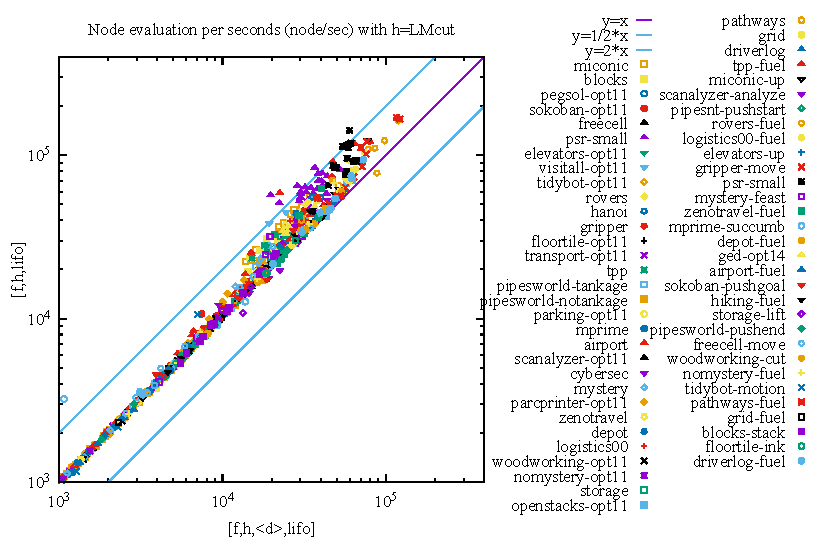
\includegraphics{img/node-sec/lmhiL-lmh_L.pdf}
 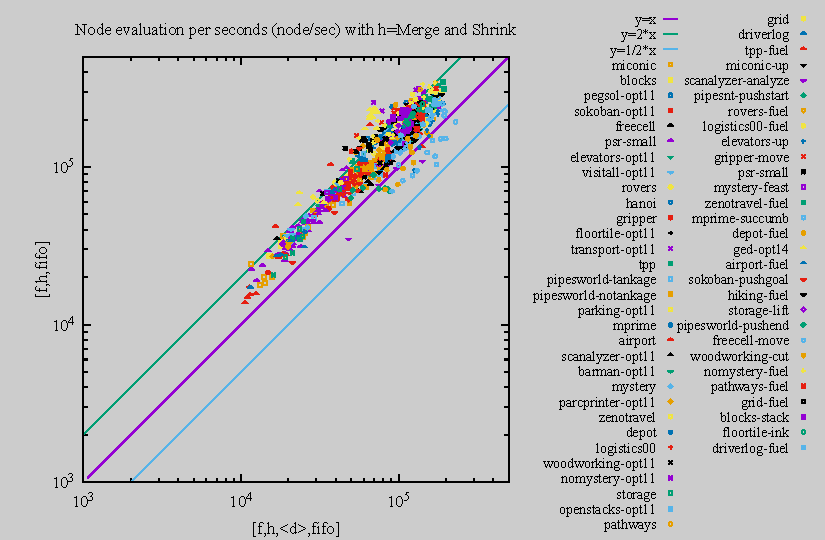
\includegraphics{img/node-sec/mnhiF-mnh_F.pdf}
 % 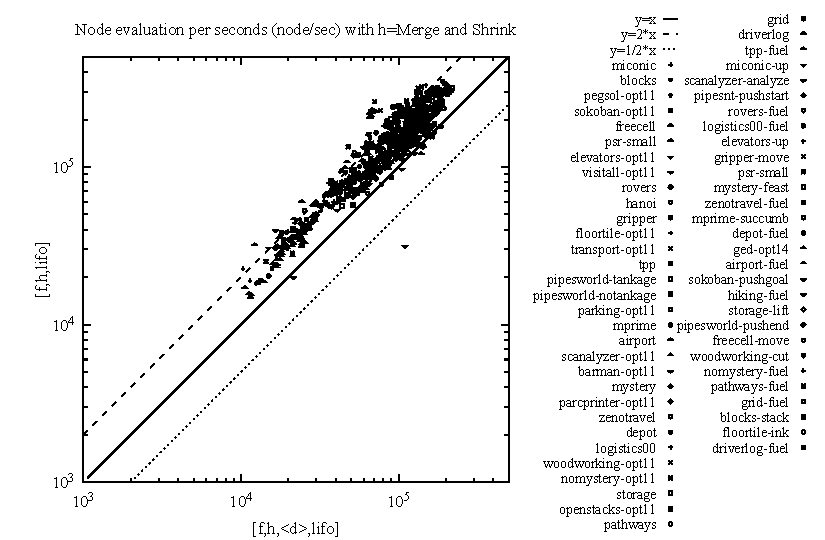
\includegraphics{img/node-sec/mnhiL-mnh_L.pdf}
 % 
 \caption{Comparison of the node evaluation ratio (node/sec) between standard tiebreaking ($y$-axis) and
 depth-based tiebreaking ($x$-axis) on \lmcut and \mands heuristics. On \mands, compared to \lmcut, node evaluation rate more often becomes
 twice as slower when depth is enabled. This is because the node evaluation of \mands is an order of
 magnitude faster than \lmcut, and the overhead of managing depth-based tiebreaking queue becomes significant. Same results were obtained with \lifo default tiebreaking. }
 % 
 \label{fig:expansion-ratio}
\end{figure}

\begin{table}[htbp]
 {
 \centering
 \let\hline\midrule
\begin{center}
\begin{tabular}{|r|*{4}{ccc|}}
 & \rb{$[f,h,\fifo]$} & \rb{$[f,h,\lifo]$} & \rb{$[f,h,\ro]$} & \rb{$[f,h,\depth,\fifo]$} & \rb{$[f,h,\depth,\lifo]$} & \rb{$[f,h,\depth,\ro]$}\\
IPC benchmark (1104) & 558 & 565 & 558.9 $\pm$ 2.1 & 571 & \textbf{575} & 571.4 $\pm$ 1.7\\
\hline
airport(50) & 27 & 26 & 25.7 $\pm$ 0.5 & 27 & 26 & 25.7 $\pm$ 0.5\\
barman-opt11(20) & 0 & 0 & 0 $\pm$ 0 & 0 & 0 & 0 $\pm$ 0\\
blocks(35) & 28 & 28 & 28 $\pm$ 0 & 28 & 28 & 28 $\pm$ 0\\
\textbf{cybersec(19)} & 2 & 3 & 3.9 $\pm$ 1.1 & 8 & \textbf{12} & 10 $\pm$ 1\\
depot(22) & 6 & 6 & 6 $\pm$ 0 & 6 & 6 & 6 $\pm$ 0\\
driverlog(20) & 13 & 13 & 13 $\pm$ 0 & 13 & 13 & 13 $\pm$ 0\\
elevators-opt11(20) & 15 & 15 & 15 $\pm$ 0 & 15 & 15 & 15 $\pm$ 0\\
floortile-opt11(20) & 6 & 6 & 6 $\pm$ 0 & 6 & 6 & 6 $\pm$ 0\\
freecell(80) & 9 & 9 & 9 $\pm$ 0 & 9 & 9 & 9 $\pm$ 0\\
grid(5) & 1 & 1 & 1 $\pm$ 0 & 1 & 1 & 1 $\pm$ 0\\
gripper(20) & 6 & 6 & 6 $\pm$ 0 & 6 & 6 & 6 $\pm$ 0\\
hanoi(30) & 12 & 12 & 12 $\pm$ 0 & 12 & 12 & 12 $\pm$ 0\\
logistics00(28) & 20 & 20 & 20 $\pm$ 0 & 20 & 20 & 20 $\pm$ 0\\
miconic(150) & 140 & 140 & 140 $\pm$ 0 & 140 & 140 & 140 $\pm$ 0\\
mprime(35) & 21 & 21 & 20.9 $\pm$ 0.3 & 21 & 21 & 20.9 $\pm$ 0.3\\
mystery(30) & 16 & 16 & 15.2 $\pm$ 0.4 & 16 & 16 & 15.4 $\pm$ 0.5\\
nomystery-opt11(20) & 14 & 14 & 14 $\pm$ 0 & 14 & 14 & 14 $\pm$ 0\\
\textbf{openstacks-opt11(20)} & 11 & \textbf{18} & 11.7 $\pm$ 0.5 & \textbf{18} & \textbf{18} & \textbf{18} $\pm$ 0\\
parcprinter-opt11(20) & 13 & 13 & 13 $\pm$ 0 & 13 & 13 & 13 $\pm$ 0\\
parking-opt11(20) & 1 & 1 & 1 $\pm$ 0 & 1 & 1 & 1 $\pm$ 0\\
pathways(30) & 5 & 5 & 5 $\pm$ 0 & 5 & 5 & 5 $\pm$ 0\\
pegsol-opt11(20) & 17 & 17 & 17 $\pm$ 0 & 17 & 17 & 17 $\pm$ 0\\
pipesworld-notankage(50) & 14 & 14 & 14.6 $\pm$ 0.5 & 14 & 15 & 14.4 $\pm$ 0.5\\
pipesworld-tankage(50) & 8 & 8 & 8 $\pm$ 0 & 8 & 8 & 8 $\pm$ 0\\
psr-small(50) & 48 & 48 & 48 $\pm$ 0 & 48 & 48 & 48 $\pm$ 0\\
rovers(40) & 7 & 7 & 7 $\pm$ 0 & 7 & 7 & 7 $\pm$ 0\\
scanalyzer-opt11(20) & 10 & 10 & 10 $\pm$ 0 & 10 & 10 & 10 $\pm$ 0\\
sokoban-opt11(20) & 19 & 19 & 19 $\pm$ 0 & 19 & 19 & 19 $\pm$ 0\\
storage(30) & 14 & 14 & 14 $\pm$ 0 & 14 & 14 & 14 $\pm$ 0\\
tidybot-opt11(20) & 12 & 12 & 12 $\pm$ 0 & 12 & 12 & 12 $\pm$ 0\\
tpp(30) & 6 & 6 & 6 $\pm$ 0 & 6 & 6 & 6 $\pm$ 0\\
transport-opt11(20) & 6 & 6 & 6 $\pm$ 0 & 6 & 6 & 6 $\pm$ 0\\
visitall-opt11(20) & 10 & 10 & 10 $\pm$ 0 & 10 & 10 & 10 $\pm$ 0\\
woodworking-opt11(20) & 10 & 10 & 10 $\pm$ 0 & 10 & 10 & 10 $\pm$ 0\\
zenotravel(20) & 11 & 11 & 11 $\pm$ 0 & 11 & 11 & 11 $\pm$ 0\\
\end{tabular}
\end{center}

  \caption{
 Coverage comparison (the number of instances solved in 5min, 4GB, LMcut
 heuristics) on \textbf{1104 standard IPC benchmark instances}. We highlight the
 best results when the difference between the maximum and the minimum coverage exceeds 2.
 }
 \label{tbl:lmcut-ipc-full}
 }
\end{table}

\begin{table}[htbp]
 {
 \centering
 \begin{center}
\begin{tabular}{|rHHHHHHHHHHHHcccHHH|cccHHH|}
\hline
 & $[f,\fifo]$ & $[f,\lifo]$ & $[f,\ro]$ & R & R & R & $[f,\depth,\fifo]$ & $[f,\depth,\lifo]$ & $[f,\depth,\ro]$ & R & R & R & $[f,h,\fifo]$ & $[f,h,\lifo]$ & $[f,h,\ro]$ & R & R & R & $[f,h,\depth,\fifo]$ & $[f,h,\depth,\lifo]$ & $[f,h,\depth,\ro]$ & R & R & R\\
\hline
IPC benchmark (1104) & 460 & 490 & 462 $\pm$ 2 & 464 & 462 & 460 & 483 & 484 & 483.3 $\pm$ 0.6 & 483 & 484 & 483 & 491 & 496 & 490 $\pm$ 1 & 491 & 490 & 489 & 487 & 487 & 485.7 $\pm$ 1.5 & 487 & 484 & 486\\
\hline
airport(50) & 9 & 9 & 9 $\pm$ 0 & 9 & 9 & 9 & 9 & 9 & 9 $\pm$ 0 & 9 & 9 & 9 & 9 & 9 & 9 $\pm$ 0 & 9 & 9 & 9 & 9 & 9 & 9 $\pm$ 0 & 9 & 9 & 9\\
barman-opt11(20) & 4 & 4 & 4 $\pm$ 0 & 4 & 4 & 4 & 4 & 4 & 4 $\pm$ 0 & 4 & 4 & 4 & 4 & 4 & 4 $\pm$ 0 & 4 & 4 & 4 & 4 & 4 & 4 $\pm$ 0 & 4 & 4 & 4\\
blocks(35) & 21 & 22 & 21 $\pm$ 0 & 21 & 21 & 21 & 21 & 22 & 21.3 $\pm$ 0.6 & 21 & 22 & 21 & 22 & 22 & 22 $\pm$ 0 & 22 & 22 & 22 & 22 & 21 & 21.7 $\pm$ 0.6 & 22 & 21 & 22\\
\textbf{cybersec(19)} & 0 & 0 & 0 $\pm$ 0 & 0 & 0 & 0 & 0 & 0 & 0 $\pm$ 0 & 0 & 0 & 0 & 0 & 0 & 0 $\pm$ 0 & 0 & 0 & 0 & 0 & 0 & 0 $\pm$ 0 & 0 & 0 & 0\\
depot(22) & 5 & 6 & 5 $\pm$ 0 & 5 & 5 & 5 & 5 & 5 & 5 $\pm$ 0 & 5 & 5 & 5 & 6 & 6 & 5 $\pm$ 0 & 5 & 5 & 5 & 5 & 5 & 5 $\pm$ 0 & 5 & 5 & 5\\
driverlog(20) & 12 & 12 & 12 $\pm$ 0 & 12 & 12 & 12 & 12 & 12 & 12 $\pm$ 0 & 12 & 12 & 12 & 12 & 12 & 12 $\pm$ 0 & 12 & 12 & 12 & 12 & 12 & 12 $\pm$ 0 & 12 & 12 & 12\\
elevators-opt11(20) & 13 & 13 & 13 $\pm$ 0 & 13 & 13 & 13 & 11 & 11 & 12 $\pm$ 0 & 12 & 12 & 12 & 13 & 13 & 13 $\pm$ 0 & 13 & 13 & 13 & 12 & 12 & 12 $\pm$ 0 & 12 & 12 & 12\\
floortile-opt11(20) & 5 & 6 & 5 $\pm$ 0 & 5 & 5 & 5 & 5 & 5 & 5 $\pm$ 0 & 5 & 5 & 5 & 6 & 6 & 6 $\pm$ 0 & 6 & 6 & 6 & 6 & 6 & 6 $\pm$ 0 & 6 & 6 & 6\\
freecell(80) & 15 & 16 & 15 $\pm$ 0 & 15 & 15 & 15 & 16 & 16 & 16 $\pm$ 0 & 16 & 16 & 16 & 17 & 17 & 16 $\pm$ 0 & 16 & 16 & 16 & 16 & 16 & 16 $\pm$ 0 & 16 & 16 & 16\\
grid(5) & 2 & 2 & 2 $\pm$ 0 & 2 & 2 & 2 & 2 & 2 & 2 $\pm$ 0 & 2 & 2 & 2 & 2 & 2 & 2 $\pm$ 0 & 2 & 2 & 2 & 2 & 2 & 2 $\pm$ 0 & 2 & 2 & 2\\
gripper(20) & 8 & 20 & 8 $\pm$ 0 & 8 & 8 & 8 & 20 & 20 & 20 $\pm$ 0 & 20 & 20 & 20 & 20 & 20 & 20 $\pm$ 0 & 20 & 20 & 20 & 20 & 20 & 20 $\pm$ 0 & 20 & 20 & 20\\
hanoi(30) & 14 & 14 & 14 $\pm$ 0 & 14 & 14 & 14 & 14 & 14 & 14 $\pm$ 0 & 14 & 14 & 14 & 14 & 14 & 14 $\pm$ 0 & 14 & 14 & 14 & 14 & 14 & 14 $\pm$ 0 & 14 & 14 & 14\\
logistics00(28) & 20 & 20 & 20 $\pm$ 0 & 20 & 20 & 20 & 20 & 20 & 20 $\pm$ 0 & 20 & 20 & 20 & 20 & 20 & 20 $\pm$ 0 & 20 & 20 & 20 & 20 & 20 & 20 $\pm$ 0 & 20 & 20 & 20\\
miconic(150) & 68 & 73 & 68.7 $\pm$ 1.2 & 70 & 68 & 68 & 73 & 73 & 73 $\pm$ 1 & 73 & 72 & 74 & 73 & 73 & 73.3 $\pm$ 0.6 & 73 & 73 & 74 & 73 & 73 & 73 $\pm$ 1 & 73 & 72 & 74\\
mprime(35) & 23 & 23 & 22.3 $\pm$ 0.6 & 22 & 22 & 23 & 23 & 23 & 23.3 $\pm$ 0.6 & 23 & 24 & 23 & 23 & 24 & 23.7 $\pm$ 0.6 & 24 & 23 & 24 & 23 & 24 & 23.7 $\pm$ 0.6 & 24 & 23 & 24\\
mystery(30) & 15 & 15 & 15 $\pm$ 0 & 15 & 15 & 15 & 15 & 15 & 15 $\pm$ 0 & 15 & 15 & 15 & 15 & 16 & 15 $\pm$ 0 & 15 & 15 & 15 & 15 & 16 & 15 $\pm$ 0 & 15 & 15 & 15\\
nomystery-opt11(20) & 17 & 18 & 18 $\pm$ 0 & 18 & 18 & 18 & 18 & 18 & 18 $\pm$ 0 & 18 & 18 & 18 & 18 & 18 & 18 $\pm$ 0 & 18 & 18 & 18 & 18 & 18 & 18 $\pm$ 0 & 18 & 18 & 18\\
\textbf{openstacks-opt11(20)} & 15 & 19 & 15.7 $\pm$ 0.6 & 16 & 16 & 15 & 19 & 19 & 19 $\pm$ 0 & 19 & 19 & 19 & 15 & 19 & 15.7 $\pm$ 0.6 & 16 & 16 & 15 & 19 & 19 & 19 $\pm$ 0 & 19 & 19 & 19\\
parcprinter-opt11(20) & 10 & 10 & 10 $\pm$ 0 & 10 & 10 & 10 & 10 & 10 & 10 $\pm$ 0 & 10 & 10 & 10 & 10 & 10 & 10 $\pm$ 0 & 10 & 10 & 10 & 10 & 10 & 10 $\pm$ 0 & 10 & 10 & 10\\
parking-opt11(20) & 1 & 1 & 1 $\pm$ 0 & 1 & 1 & 1 & 1 & 1 & 1 $\pm$ 0 & 1 & 1 & 1 & 1 & 1 & 1 $\pm$ 0 & 1 & 1 & 1 & 1 & 1 & 1 $\pm$ 0 & 1 & 1 & 1\\
pathways(30) & 4 & 4 & 4 $\pm$ 0 & 4 & 4 & 4 & 4 & 4 & 4 $\pm$ 0 & 4 & 4 & 4 & 4 & 4 & 4 $\pm$ 0 & 4 & 4 & 4 & 4 & 4 & 4 $\pm$ 0 & 4 & 4 & 4\\
pegsol-opt11(20) & 17 & 19 & 17.3 $\pm$ 0.6 & 17 & 18 & 17 & 18 & 19 & 19 $\pm$ 0 & 19 & 19 & 19 & 19 & 19 & 19 $\pm$ 0 & 19 & 19 & 19 & 19 & 19 & 19 $\pm$ 0 & 19 & 19 & 19\\
pipesworld-notankage(50) & 9 & 9 & 8.7 $\pm$ 0.6 & 9 & 9 & 8 & 10 & 9 & 8.7 $\pm$ 0.6 & 9 & 9 & 8 & 10 & 10 & 9.7 $\pm$ 0.6 & 10 & 10 & 9 & 10 & 9 & 9.7 $\pm$ 0.6 & 10 & 10 & 9\\
pipesworld-tankage(50) & 13 & 13 & 13.3 $\pm$ 0.6 & 14 & 13 & 13 & 13 & 13 & 13 $\pm$ 0 & 13 & 13 & 13 & 13 & 13 & 13.7 $\pm$ 0.6 & 14 & 14 & 13 & 13 & 13 & 13 $\pm$ 0 & 13 & 13 & 13\\
psr-small(50) & 50 & 50 & 50 $\pm$ 0 & 50 & 50 & 50 & 50 & 50 & 50 $\pm$ 0 & 50 & 50 & 50 & 50 & 50 & 50 $\pm$ 0 & 50 & 50 & 50 & 50 & 50 & 50 $\pm$ 0 & 50 & 50 & 50\\
rovers(40) & 6 & 8 & 6 $\pm$ 0 & 6 & 6 & 6 & 8 & 8 & 7 $\pm$ 0 & 7 & 7 & 7 & 8 & 8 & 8 $\pm$ 0 & 8 & 8 & 8 & 8 & 8 & 7 $\pm$ 0 & 7 & 7 & 7\\
scanalyzer-opt11(20) & 10 & 10 & 10 $\pm$ 0 & 10 & 10 & 10 & 10 & 10 & 10.3 $\pm$ 0.6 & 10 & 10 & 11 & 10 & 10 & 10 $\pm$ 0 & 10 & 10 & 10 & 10 & 10 & 10 $\pm$ 0 & 10 & 10 & 10\\
sokoban-opt11(20) & 20 & 20 & 20 $\pm$ 0 & 20 & 20 & 20 & 19 & 19 & 18.7 $\pm$ 0.6 & 19 & 19 & 18 & 20 & 20 & 20 $\pm$ 0 & 20 & 20 & 20 & 19 & 19 & 18.7 $\pm$ 0.6 & 19 & 19 & 18\\
storage(30) & 15 & 15 & 15 $\pm$ 0 & 15 & 15 & 15 & 15 & 15 & 15 $\pm$ 0 & 15 & 15 & 15 & 15 & 15 & 15 $\pm$ 0 & 15 & 15 & 15 & 15 & 15 & 15 $\pm$ 0 & 15 & 15 & 15\\
tidybot-opt11(20) & 0 & 0 & 0 $\pm$ 0 & 0 & 0 & 0 & 0 & 0 & 0 $\pm$ 0 & 0 & 0 & 0 & 0 & 0 & 0 $\pm$ 0 & 0 & 0 & 0 & 0 & 0 & 0 $\pm$ 0 & 0 & 0 & 0\\
tpp(30) & 6 & 6 & 6 $\pm$ 0 & 6 & 6 & 6 & 6 & 6 & 6 $\pm$ 0 & 6 & 6 & 6 & 7 & 6 & 6 $\pm$ 0 & 6 & 6 & 6 & 6 & 6 & 6 $\pm$ 0 & 6 & 6 & 6\\
transport-opt11(20) & 7 & 7 & 7 $\pm$ 0 & 7 & 7 & 7 & 6 & 6 & 6 $\pm$ 0 & 6 & 6 & 6 & 7 & 7 & 7 $\pm$ 0 & 7 & 7 & 7 & 6 & 6 & 6 $\pm$ 0 & 6 & 6 & 6\\
visitall-opt11(20) & 9 & 9 & 9 $\pm$ 0 & 9 & 9 & 9 & 9 & 9 & 9 $\pm$ 0 & 9 & 9 & 9 & 9 & 9 & 9 $\pm$ 0 & 9 & 9 & 9 & 9 & 9 & 9 $\pm$ 0 & 9 & 9 & 9\\
woodworking-opt11(20) & 7 & 7 & 7 $\pm$ 0 & 7 & 7 & 7 & 7 & 7 & 7 $\pm$ 0 & 7 & 7 & 7 & 7 & 7 & 7 $\pm$ 0 & 7 & 7 & 7 & 7 & 7 & 7 $\pm$ 0 & 7 & 7 & 7\\
zenotravel(20) & 10 & 10 & 10 $\pm$ 0 & 10 & 10 & 10 & 10 & 10 & 10 $\pm$ 0 & 10 & 10 & 10 & 12 & 12 & 12 $\pm$ 0 & 12 & 12 & 12 & 10 & 10 & 10 $\pm$ 0 & 10 & 10 & 10\\
\hline
\end{tabular}
\end{center}

  \caption{
 Coverage comparison (the number of instances solved in 5min, 4GB, M\&S
 heuristics) on \textbf{1104 standard IPC benchmark instances}. We highlight the
 best results when the difference between the maximum and the minimum coverage exceeds 2.
 }
 \label{tbl:mands-ipc-full}
 }
\end{table}

% \reftbl{tbl:mands-evaluations} shows that if we instead compare the
% number of evaluations on problems solved by both, depth-based
% tiebreaking significantly outperforms the standard tiebreaking
% strategies. Moreover, in the next \textbf{zerocost} domain experiments,
% depth-based tiebreaking ourperforms the standard tiebreaking
% overall. Besides, the coverages by \mands is less than that of \lmcut.

% \begin{figure}[htb]
%  \centering
%  \caption{
%  Comparison of the total number of nodes generated
%  by \mands heuristics until
%  the goal is found, with vs without depth-based tiebreaking.
%  } \label{tbl:mands-evaluations}
% \end{figure}

\clearpage

\subsection{Search Behavior Within a Plateau}

To understand the behavior of depth-based policies, we plotted 
histograms of the depths of search nodes evaluated by several tiebreaking
strategies in the final plateau $\plateau{f^*,0}$ until the solution is
found.  We plotted the most successful depth-based strategy,
$[f,h,\depth,\fifo]$, as well as the standard strategies $[f,h,\fifo]$,
$[f,h,\lifo]$ and a single run of randomized strategy $[f,h,\ro]$.

In addition, we  added some instrumentation to the strategies which do not use depth-based tiebreaking ($[f,h,\fifo]$, $[f,h,\lifo]$, $[f,h,\ro]$) so that as these strategies run, the depth of each of the expanded nodes is computed (although they do not affect the search behavior).
Note that this instrumentation, which adds some runtime overhead, was \emph{not}
used in the performance comparison experiments above, and were only used for this experiment, which analyzes search behavior.


\refigs{fig:depth-histogram}{fig:depth-histogram3} show the results on several exemplar instances in
various zerocost domains.  We do not show some domains when we did not observe any depths more than 3, where
the depth metric has negligible effect on the search performance.

In many domains, we observed that the depth-first behavior of
$[f,h,\lifo]$ results in deeper search, missing the key branch at
intermediate depths.  On the other hand, the breadth-first behavior of
$[f,h,\fifo]$ often gets stuck spending an excessive amount of time
searching around the plateau entrance.  Also, due to the large bias of
the number of nodes to the shallower depths, global randomization
$[f,h,\ro]$ showed a distribution similar to $[f,h,\fifo]$.
In contrast, $[f,h,\depth,\ro]$ is balancing the search at various depths, which
results in successfully solving more problems.\todo{Instead of only general trends for unspecified domains, mentioning specific domains to add some ``color'' might make this more interesting}

Moreover, the results in \refigs{fig:depth-histogram}{fig:depth-histogram3} suggest that in many domains the distribution of $[f,h,\depth,\ro]$ follows
$D-d$, a theoretical formula which was made under the simplified
assumption that the plateau forms a tree of fixed branching factor. In these
figures, $D$ means the largest depth in the open list, which is equal to
the number of iterations that has ever happened in the depth diversification framework.\todo{refs to sec{sec:theoretical-characteristics}}

The discrepancy from the theoretical prediction can be caused by the 
following factors: First, the branching factor of the graph may not be
uniform across the search space. Second, some depth buckets could be
exhausted, as is depicted in the line by $[f,h,\fifo]$ which
shows all nodes in the shallower depths are expanded and the line can be below $D-d$.

Next, \refig{fig:depth-histogram4} shows the same results on the standard IPC
Openstacks and Cybersec domains.
The result in Openstacks was similar to those of the zerocost domains.
In Cybersec,
% while the depth has improved the overall performance,
we found that the performance improvement was not due to the number of nodes in $\plateau{f^*,0}$ because it was small\footnote{This does not contradict to the results in \refig{fig:plateau} because \refig{fig:plateau} uses a modified Fast Downward which continues the search until expanding all nodes in the final plateau, while in this experiment the planner immediately stops the search after the first solution. These figures are supposed to serve the different experimental purposes: \refig{fig:plateau} was intended to show the size of the entire final plateau, while \refig{fig:depth-histogram} to \refig{fig:depth-histogram4} was meant to show the actual search behavior. If we were to continue the search after the first solution, all tiebreaking strategies should result in the same figure because they expands the same set of nodes.} according to the plot.
Instead, we observed a large difference in the depth distribution in $\plateau{f^*,1}$ caused by the difference of tiebreaking (\refig{fig:depth-histogram5}), which shows that the depth can also enhance the search in non-final plateaus to find the nodes in the next plateau.
Similar phenomena were observed in several domains (which are included in \refig{fig:depth-histogram5}).\todo{if it's only ``several'', might as well say which domains instead of having the reader figure it out. Similarly, throughout this subsection and elsewhere, consider giving more specific info (domain names, or number of domains) whenever words like ``some/several/various'' are used}


\begin{figure}[htbp]
% 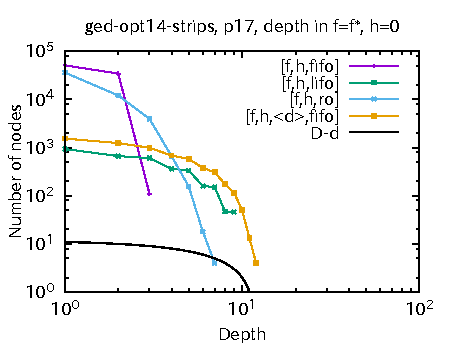
\includegraphics{img/output-lmcut/ged-opt14-strips/p17.pdf}
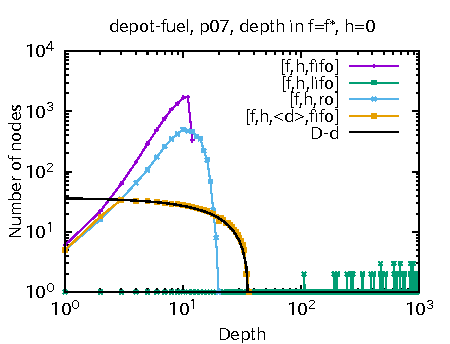
\includegraphics{img/output-lmcut/depot-fuel/p07.pdf}
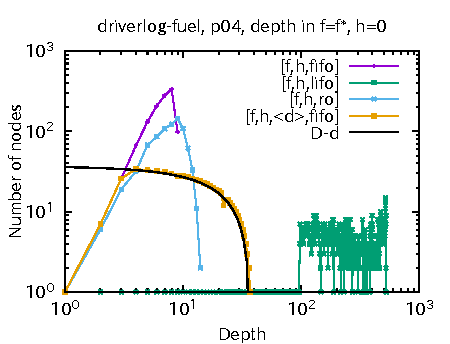
\includegraphics{img/output-lmcut/driverlog-fuel/p04.pdf}
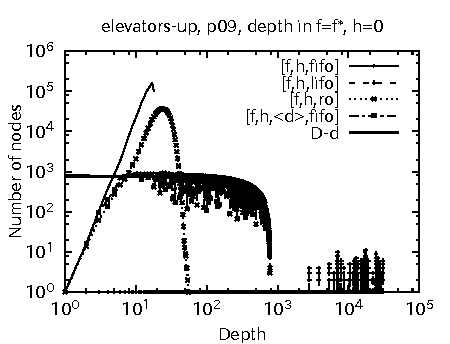
\includegraphics{img/output-lmcut/elevators-up/p09.pdf}
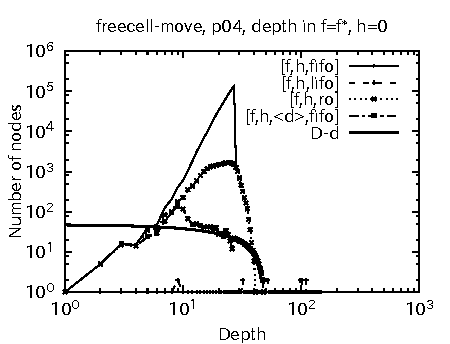
\includegraphics{img/output-lmcut/freecell-move/p04.pdf}
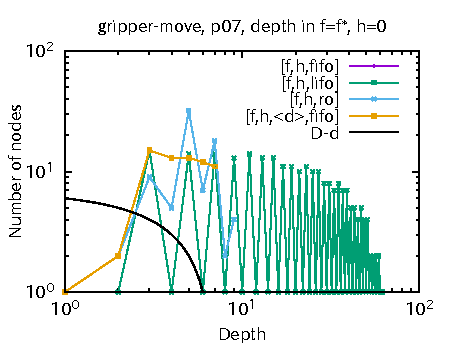
\includegraphics{img/output-lmcut/gripper-move/p07.pdf}
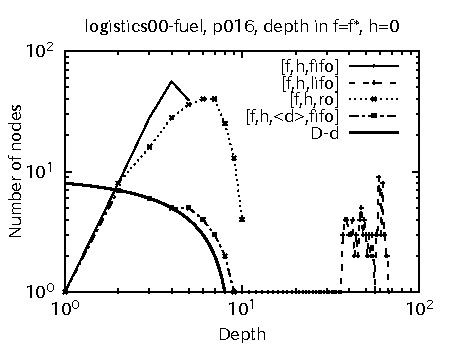
\includegraphics{img/output-lmcut/logistics00-fuel/p016.pdf}
 \caption{(Page 1/4) Number of nodes ($y$-axis) expanded per depth ($x$-axis) in
 the final plateau with different tiebreakings. Both axes are in logarithmic scale.
 }
 \label{fig:depth-histogram}
\end{figure}

\begin{figure}[htbp]
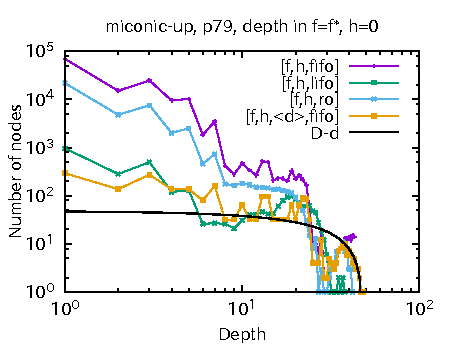
\includegraphics{img/output-lmcut/miconic-up/p79.pdf}
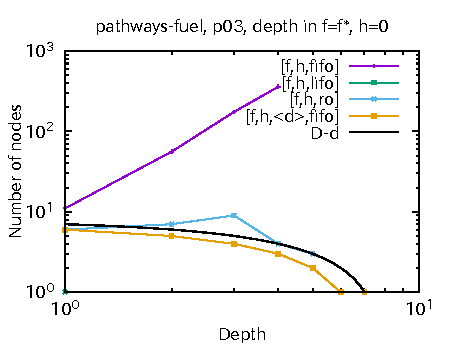
\includegraphics{img/output-lmcut/pathways-fuel/p03.pdf}
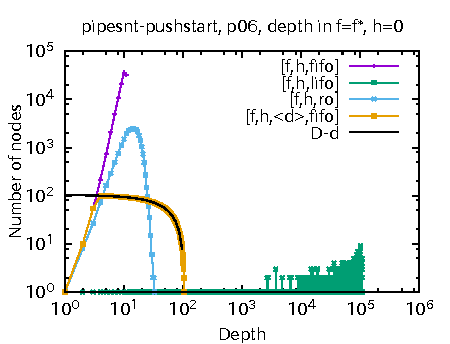
\includegraphics{img/output-lmcut/pipesnt-pushstart/p06.pdf}
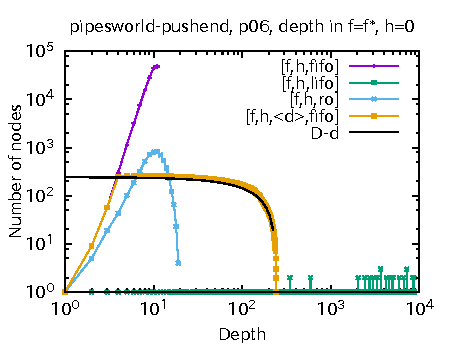
\includegraphics{img/output-lmcut/pipesworld-pushend/p06.pdf}
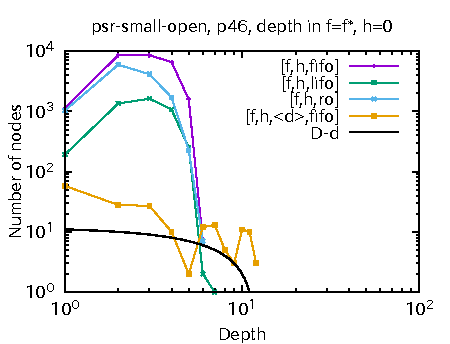
\includegraphics{img/output-lmcut/psr-small-open/p46.pdf}
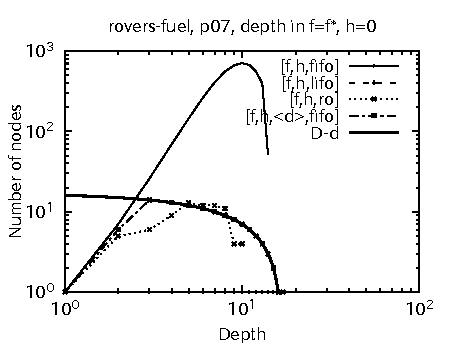
\includegraphics{img/output-lmcut/rovers-fuel/p07.pdf}
 \caption{(Page 2/4) Number of nodes ($y$-axis) expanded per depth ($x$-axis) in
 the final plateau with different tiebreakings. Both axes are in logarithmic scale.
 }
 \label{fig:depth-histogram2}
\end{figure}

\begin{figure}[htbp]
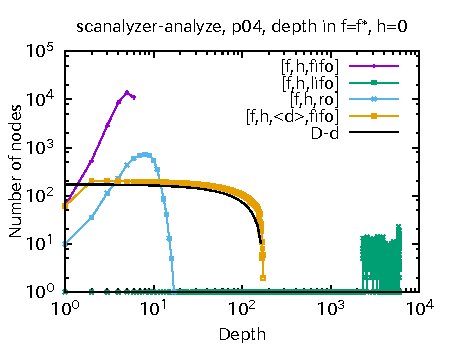
\includegraphics{img/output-lmcut/scanalyzer-analyze/p04.pdf}
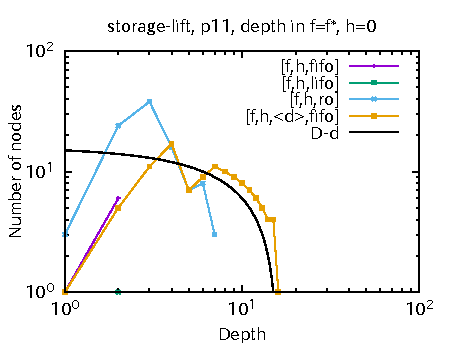
\includegraphics{img/output-lmcut/storage-lift/p11.pdf}
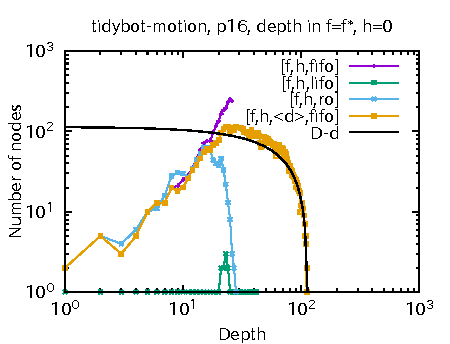
\includegraphics{img/output-lmcut/tidybot-motion/p16.pdf}
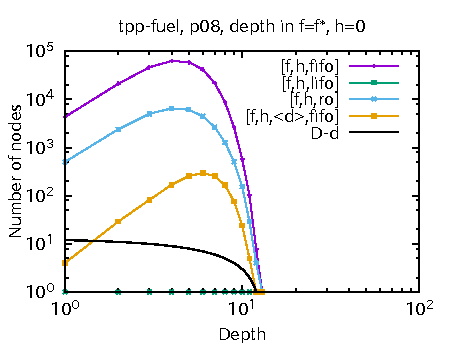
\includegraphics{img/output-lmcut/tpp-fuel/p08.pdf}
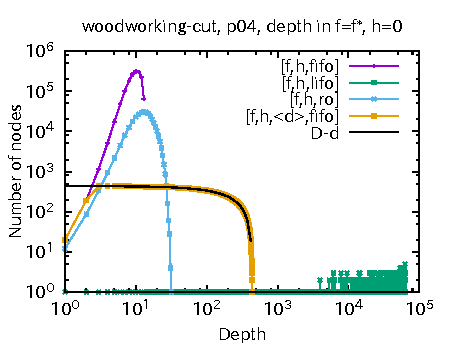
\includegraphics{img/output-lmcut/woodworking-cut/p04.pdf}
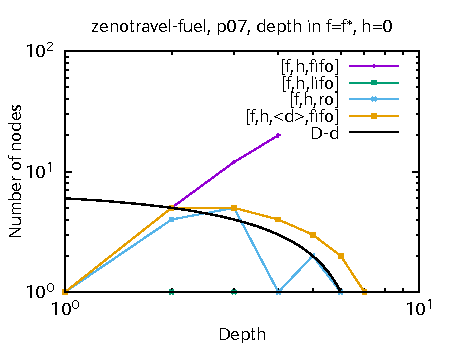
\includegraphics{img/output-lmcut/zenotravel-fuel/p07.pdf}
 \caption{(Page 3/4) Number of nodes ($y$-axis) expanded per depth ($x$-axis) in
 the final plateau with different tiebreakings. Both axes are in logarithmic scale.
 }
 \label{fig:depth-histogram3}
\end{figure}

\begin{figure}[htbp]
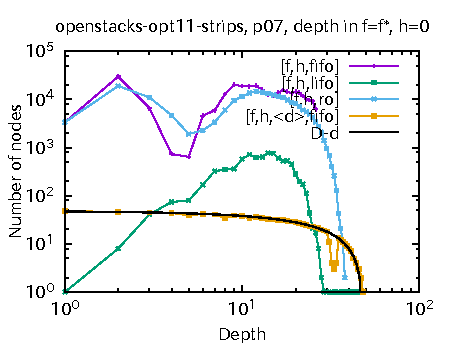
\includegraphics{img/output-lmcut/openstacks-opt11-strips/p07.pdf}
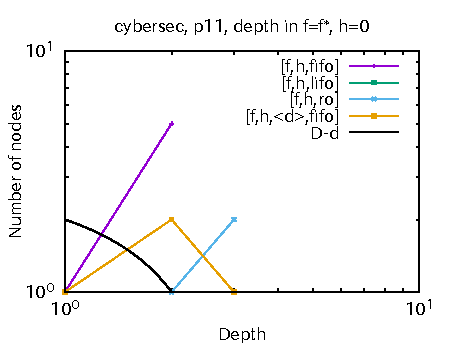
\includegraphics{img/output-lmcut/cybersec/p11.pdf}
 \caption{(Page 4/4) Depth distribution in the final plateau ($\plateau{f^*,0}$).}
 \label{fig:depth-histogram4}
\end{figure}

\begin{figure}[htbp]
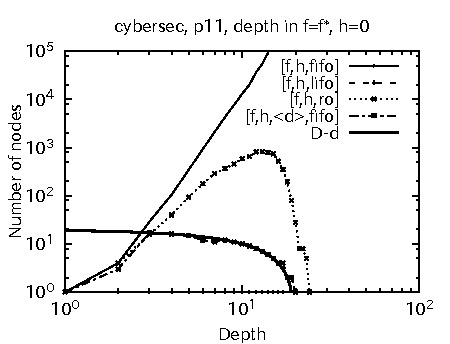
\includegraphics{img/output-lmcut1/cybersec/p11.pdf}
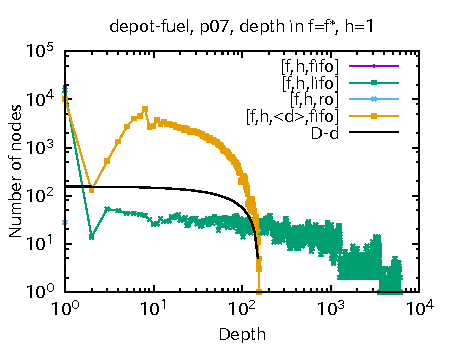
\includegraphics{img/output-lmcut1/depot-fuel/p07.pdf}
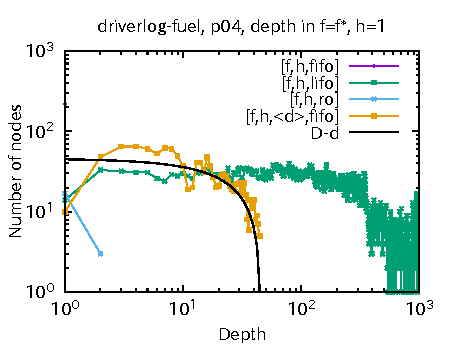
\includegraphics{img/output-lmcut1/driverlog-fuel/p04.pdf}
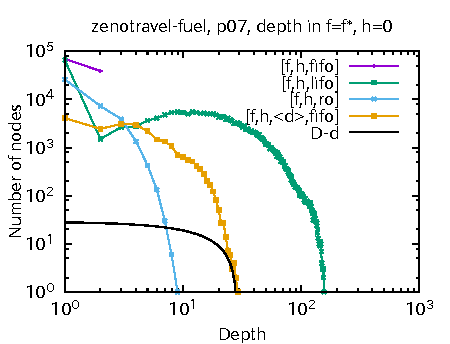
\includegraphics{img/output-lmcut1/zenotravel-fuel/p07.pdf}
 \caption{Depth distribution in a non-final plateau ($\plateau{f^*,1}$).}
 \label{fig:depth-histogram5}
\end{figure}

